\documentclass[11pt]{article} % The style of the article, and font size
\oddsidemargin -0.0in
\topmargin -0.5in
\usepackage{algorithm}
\usepackage[noend]{algpseudocode}
\usepackage{mathtools}
\usepackage{amsfonts}
\usepackage{float}
\usepackage{physics} %my preferred \abs{} 
\usepackage{graphicx}
\textwidth 6.25in
\textheight 9.25in
\setlength\parindent{1cm} % Sets the indentation for new paragraphs.

\begin{document}

\title{Analysis of Multi-threading Matrix Multiplication}
\author{Michael Albert}
\date{June 06, 2019}
\maketitle

\section*{Implementation}
To add threading to the matrix multiplication program, a struct was added which contained relevant information for the multiplication (pointers to A,B, and C, size of x,y,z, number of threads, thread number, and number of times to multiply the matrix). An array of structs were created and the info was filled out in the calls to MatMul and MatSquare. These were passed in as the thread body argument.

From there, the thread body called a helper function called matrix\_calc. This function used the thread number and number of threads to determine and then calculate the elements of the final array that a given thread should do. For MatMul, the only other thing that is needed is a loop to join all the threads after they finish the calculations.

For MatSquare, thread synchronization is also required. A barrier was implemented and pthread\_barrier\_wait was called once for every additional call to matrix\_calc. After this, all that is needed is to join all the threads and destroy the barrier.

\section*{Experiments}
Our goal was to determine the relative decrease in the computational time required to multiply matrices when using threads versus when not. We define the 'speedup' as the the time taken without threads divided by the time taken with. In the experiments, we multiply matrices of dimension 1500, 1750, and 2000, and compute the time taken without threads and with $n$ threads, where $n$ is between 2 and 16. We then raise matrices of dimension 1000, 1150, and 1300 to the sixth power and compute the time taken.

A simple bash script was created to run and record the output of the multiplications, with the speedup then being calculated. To create a more consistent output, test runs were repeated five times with the average being used to calculate the speedup. 

\begin{figure}
\centering
\begin{minipage}{.5\textwidth}
  \centering
  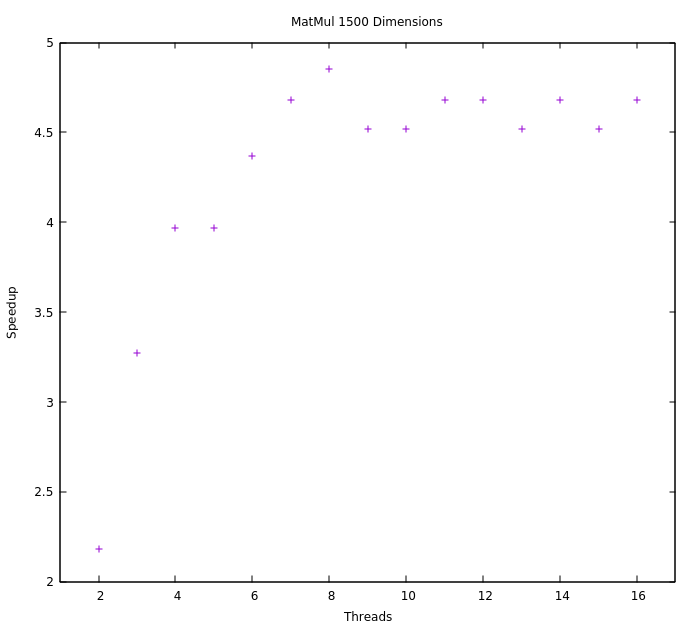
\includegraphics[width=1\linewidth]{MatMul1.png}
  \label{fig:test1}
\end{minipage}%
\begin{minipage}{.5\textwidth}
  \centering
  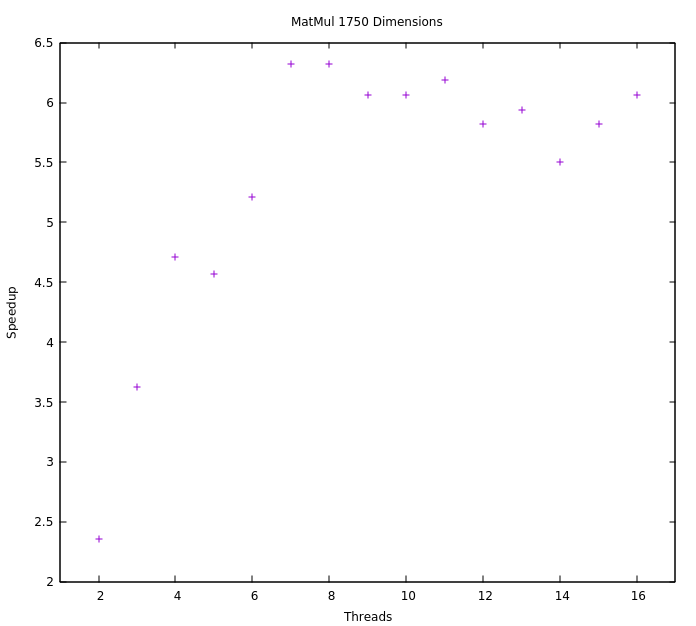
\includegraphics[width=1\linewidth]{MatMul2.png}
  \label{fig:test2}
\end{minipage}
\end{figure}

\begin{figure}
\centering
\begin{minipage}{.5\textwidth}
  \centering
  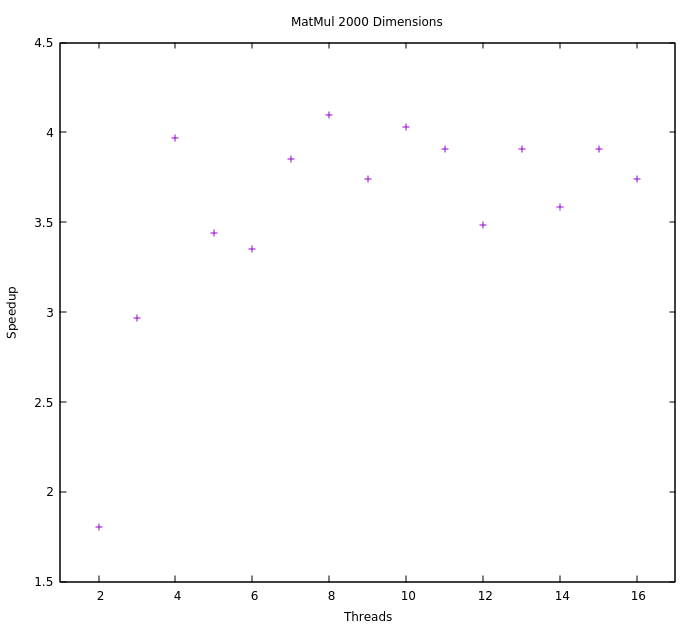
\includegraphics[width=1\linewidth]{MatMul3.png}
  \label{fig:test3}
\end{minipage}%
\begin{minipage}{.5\textwidth}
  \centering
  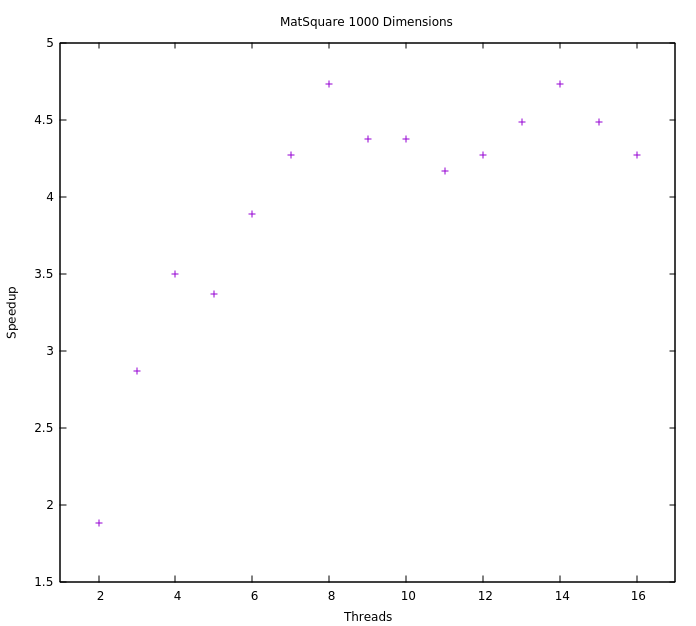
\includegraphics[width=1\linewidth]{MatSquare1.png}
  \label{fig:test4}
\end{minipage}
\end{figure}

\begin{figure}
\centering
\begin{minipage}{.5\textwidth}
  \centering
  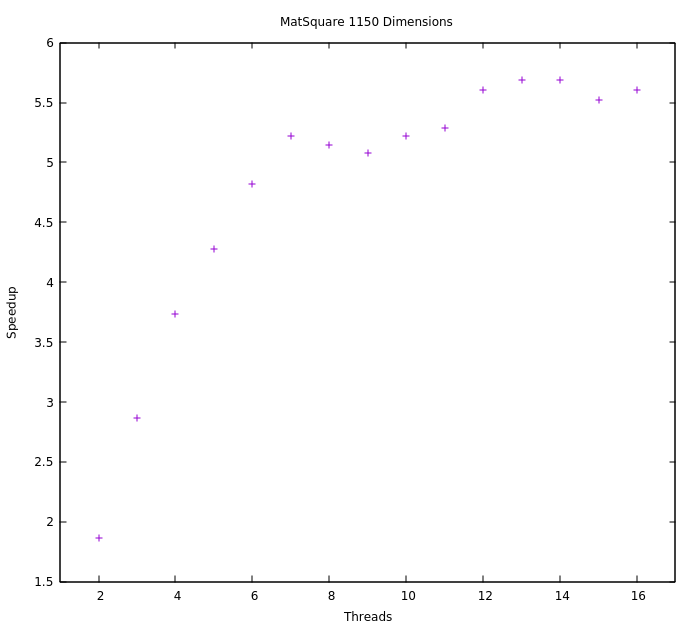
\includegraphics[width=1\linewidth]{MatSquare2.png}
  \label{fig:test5}
\end{minipage}%
\begin{minipage}{.5\textwidth}
  \centering
  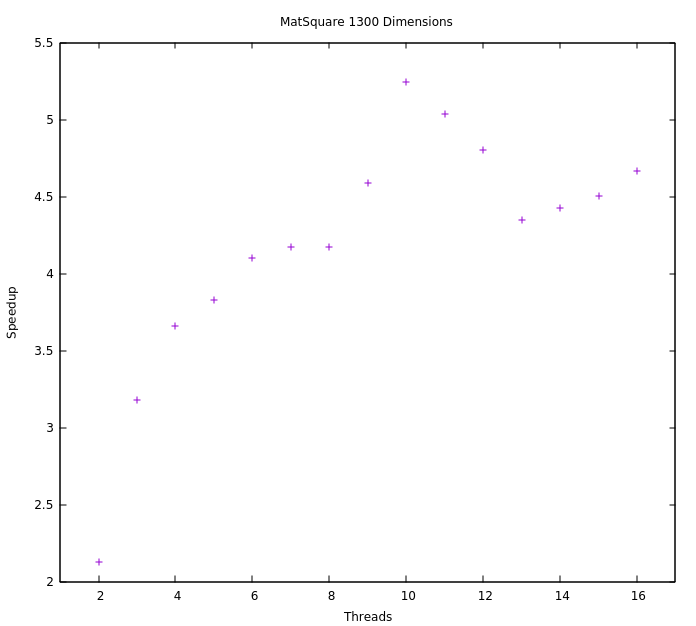
\includegraphics[width=1\linewidth]{MatSquare3.png}
  \label{fig:test6}
\end{minipage}
\end{figure}

\newpage

\section*{Results}
As can be seen in the graphs, there was a substantial increase in speedup time when using between 2 and 8 threads. We also note that there after the initial jumps between threads 2 through 8, the speedup time remains relatively stable. We note that the graphs stabilize between 4 and 6, indicating that the threaded implementation was able to calculate the results 4 to 6 times as quickly as the non-threaded version.

We also see that at a certain threshold, introducing more threads does not improve the time and, indeed, seems to potentially lower the speedup. This seems like reasonable behavior since once the number of threads used exceeds the number of cores that a computer can run the threads on, the work is no longer being done in parallel. We then expect it will take a similar amount of time as it would with threads equal to the number of cores while also incurring the overhead cost of the additional threads.

\section*{Conclusion}
It is clear that multi-threading is a powerful tool to use when dealing with large computations that can be separated into parts and computed simultaneously. Examining the results, it seems to me that threads are, while not easy to use, a helpful way to get large decreases in the run time of many different types of programs. Learning how to use threads in a safe and reliable manner is something that will likely become more and more important for programmers as the speed with which a computer can do sequential calculations starts to hit a maximum limit. 

\end{document}